Figure \ref{fig:idf-syntax} shows the full syntax of \svlidf.
\begin{figure}[h]
    \newcommand{\tempStmtA}{\sSkip
                    ~|~ \sDeclare {$T$} {$x$}
                    ~|~ \sFieldAssign {$x$} {$f$} {$y$} 
                    ~|~ \sVarAssign {$x$} {$e$}
                    ~|~ \sAlloc {$x$} {$C$} 
                    ~|~ \sCall {$x$} {$y$} {$m$} {$z$}}
\newcommand{\tempStmtB}{~~~ ~|~ \sReturn {$x$}  
                            ~|~ \sAssert {$\phi$} 
                            ~|~ \sRelease {$\phi$} 
                            ~|~ \sHold {$\phi$} {$s$}
                            ~|~ \sSeq {$s_1$} {$s_2$}}
\newcommand{\tempFrm}{  \phiTrue 
                    ~|~ \phiEq {$e$} {$e$} 
                    ~|~ \phiNeq {$e$} {$e$}
                    ~|~ \phiAcc {$e$} {$f$}
                    ~|~ \phiCons {$\phi$} {$\phi$}}
\newcommand{\tempExpr}{ \ev{$v$}
                    ~|~ \ex{$x$}
                    ~|~ \edot{$e$}{$f$}}

\begin{align*}
	program  & \in \setProgram    &  & ::= \ttt{$\overline{cls}$~$\overline{s}$}                         \\
	cls      & \in \setClass      &  & ::= \class {$C$} {$\overline{field}$} {$\overline{method}$}       \\
	field    & \in \setField      &  & ::= \field {$T$} {$f$}                                            \\
	method   & \in \setMethod     &  & ::= \method {$T$} {$m$} {$T$} {$x$} {$contract$} {$\overline{s}$} \\
	contract & \in \setContract   &  & ::= \ttt{requires $\phi$;~ensures $\phi$;}                        \\
	T        & \in \setType       &  & ::= \Tint ~|~ C                                                   \\
	s        & \in \setStmt       &  & ::= \tempStmtA                                                    \\
	         &                    &  & \tempStmtB                                                        \\
	\phi     & \in \setFormula    &  & ::= \tempFrm                                                      \\
	e        & \in \setExpr       &  & ::= \tempExpr                                                     \\
	x, y, z  & \in \setVar        &  & ::= \ethis ~|~ \eresult ~|~ name                                  \\
	v        & \in \setVal        &  & ::= o ~|~ n ~|~ \enull                                            \\
	o        & \in \setObj        &  &  \\
	n        & \in \mathbb{Z}     &  &  \\
	C        & \in \setClassName  &  & ::= name                                                          \\
	f        & \in \setFieldName  &  & ::= name                                                          \\
	m        & \in \setMethodName &  & ::= name
\end{align*} 
    \caption{\svlidf: Syntax}
    \label{fig:idf-syntax}
\end{figure}
% EXPLAIN what stuff (like hold, release) means!

%% parser rassoc, skip
We define $\ttt{;}$ to be right-associative and assume that parsing a sequence of statements (e.g. method body) operates analogously, obviating the need for parenthesis.
Furthermore we assume that the parser terminates every sequence with $\sSkip$.
\begin{exmp}~
    \begin{lstlisting}
    ...
    {
        $s_1$;
        $s_2$;
        $s_3$;
    }
    \end{lstlisting}
    is parsed as
    
    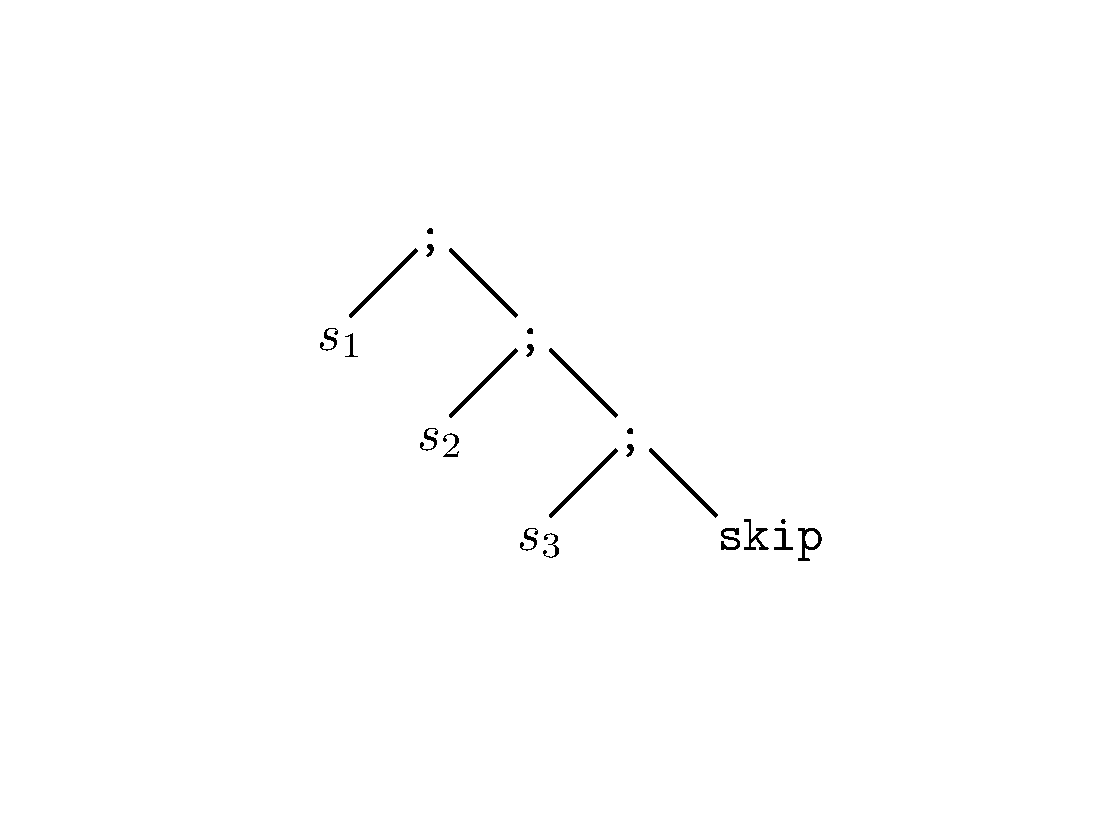
\includegraphics[trim={3cm 3cm 3cm 3cm}, clip, width=6cm]{graphics/rightAssocSkip}
\end{exmp}
These assumptions highly simplify reasoning about statements.
